\documentclass[12pt,a4paper]{article}
\usepackage[utf8]{inputenc}
\usepackage[english,finnish]{babel}
\usepackage{amsmath}
\usepackage{amsfonts}
\usepackage{amssymb}
\usepackage{graphicx}
\usepackage[left=2cm,right=2cm,top=2cm,bottom=2cm]{geometry}
\usepackage{hyperref}

\title{Projektinhallintajärjestelmä\\Toteutusdokumentti}

\author{Markus Korpinen}

\begin{document}
\maketitle
\section*{Johdanto}
Toteutetaan projektinhallintajärjestelmä, jonka avulla voidaan seurata eri projektien etenemistä. Käyttäjät voivat kirjautumisen jälkeen luoda omia projekteja ja jakaa niitä muiden käyttäjien kanssa. Projektien alle voidaan asettaa  tehtäviä eri prioriteeteillä ja aikatauluilla. Projektinhallintajärjestelmä toteutetaan käyttäen Ruby-kieltä ja MVC-malliin pohjautuvaa Ruby on Rails -ohjelmistokehystä. Tietokantannaksi valitaan PostgreSQL ja Web-palvelimeksi WebRICK. Versionhallintana käytetään gitiä ja ohjelmisto julkaistaan Heroku.com palvelussa.
\section*{Rajaukset}
Lisättiin tietokantaan \textit{sessions}--taulu, joka huolehtii käyttäjien järjestelmään kirjautumisesta.

\section*{Ohjelmiston yleisrakenne}
Kuten kaikki Rails-ohjelmistot, järjestelmä käyttää MVC-arkkitehtuuria, eli koostuu
malleista (Models), näkymistä (Views) ja käsittelijöistä (Controllers).

Näkymät kuvaavat järjestelmän tiedon tallentamisen ja muun käsittelyn, eli vastaavat
tietokannan tauluja. Näkymät vastaavat tietojen esittämisestä käyttöliittymässä. Käsittelijät
taas vastaanottavat käyttäjältä tulevat pyynnöt ja hakevat tarvittavat tiedot mallilta ja
lähettävät ne näkymille.

\begin{figure}[h!]
	\centering
	\caption{Järjestelmän MVC-komponentit}
	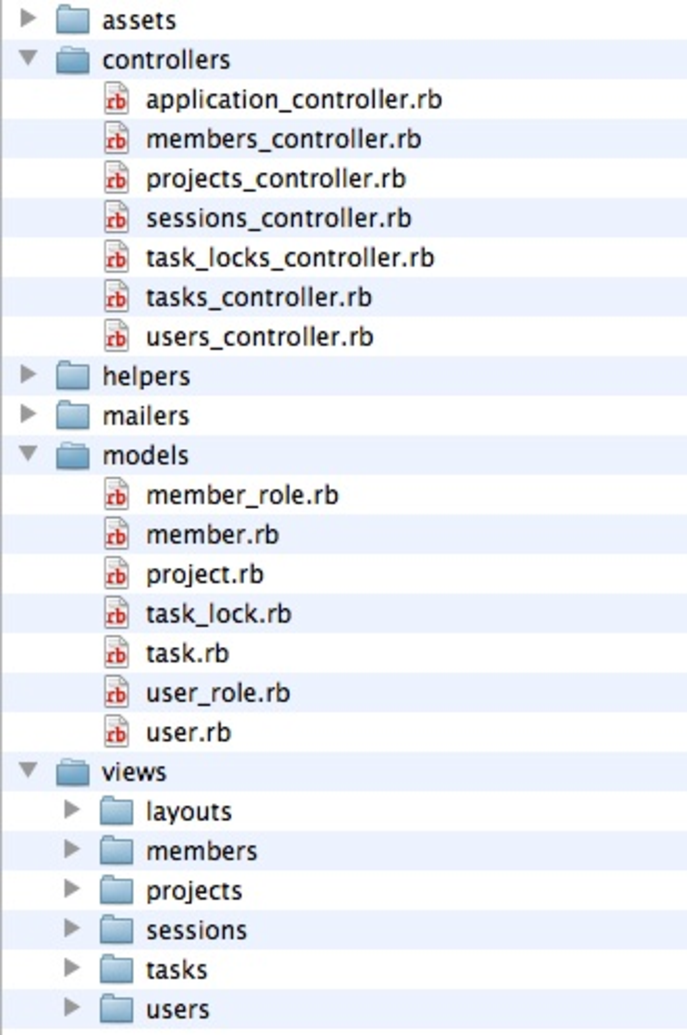
\includegraphics[width=0.45\textwidth]{mvc.pdf}
	%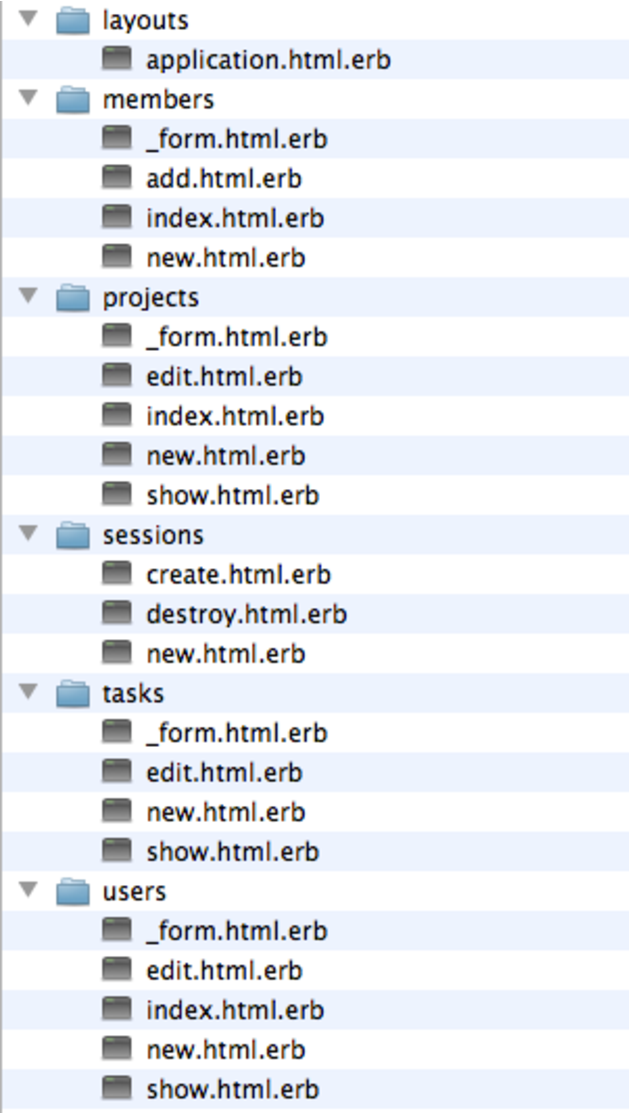
\includegraphics[width=0.45\textwidth]{mvc2.pdf}
\end{figure}


\section*{Järjestelmän komponentit}
\subsection*{Mallit (models)}
Mallin jälkeen suluissa mallia vastaavan tietokantataulun kentät.
Kaikissa tauluissa mainittujen kenttien lisäksi kentät created\_at:datetime ja
updated\_at:datetime.
\subsubsection*{Member}
(project\_id:int, user\_id:int, member\_role\_id:int, title:string)\\\\
Tauluun tallennetaan kunkin projektin jäsenet. Viittaukset projektiin, käyttäjään ja jäsenrooliin.
\subsubsection*{MemberRole}
(role:string)\\\\
Taulussa tallennettuna projektin jäsenen roolit, kuten ”creator” tai ”user”.
\subsubsection*{Project}
(name:string, url:string, description:text, visibility:string, deadline:datetime)\\\\
Vaaditut kentät ovat name ja deadline.
Mallissa huolehditaan, että projektia poistettaessa poistetaan samalla kaikki projektin
tehtävät ja jäsenet.
\subsubsection*{Task}
(project\_id:int, description:text, priority:int, status:string, deadline:datetime,
comment:string, name:string)\\\\
Tehtävää poistettaessa poistetaan samalla kaikki tehtävään liittyvät lukot (task\_locks).
Tehtävässä viittaus projektiin.
\subsubsection*{TaskLock}
(task\_id:int, user\_id:int)\\\\
Viittaukset tehtävään ja käyttäjään.
Projektin hallinnoijan allokoidessa tehtävän projektin jäsenelle, luodaan uusi rivi
task\_locks-tauluun.
\subsubsection*{User}
(user\_role\_id:int, username:string, email:string, password\_salt:string,
encrypted\_password:string)\\\\
Malli huolehtii uuden käyttäjän luonnista tietokantaan. Salasana kryptataan suolattuna
SHA2--algoritmia käyttäen.
\subsubsection*{UserRole}
(role:string)\\\\
Taulussa tallennettuna järjestelmän käyttäjien roolit, kuten ”administrator”.
\subsection*{Käsittelijät (controllers)}
Käsittelijän jälkeen suluissa käsittelijän metodit (protected tai private hakasuluissa).
\subsubsection*{ApplicationController}
([logged\_in?], [authorize], [is\_admin?], [can\_add?])\\\\
Käsittelijän metodit tarkistavat käyttäjän sisäänkirjautumisen tilan ja huolehtivat
käyttöoikeuksien myöntämisestä riippuen siitä, onko käyttäjä jonkin projektin jäsen, tai
onko käyttäjällä hallinnointioikeudet projektiin.
\subsubsection*{MembersController}
(index, add, new, create)\\\\
Index-metodia lukuunottamatta ApplicationController\#can\_add?-metodi tarkastaa ennen
käsittelijän metodikutsuja voiko käyttäjä lisätä uusia jäseniä projektiin, eli onko käyttäjä
joko projektin luoja tai hallinnoija.
Add-metodi luo instanssimuuttujan @users, jossa on kaikki järjestelmän käyttäjät, jotka
eivät vielä ole projektin jäseniä. Tämä muuttuja välitetään vastaavalle näkymälle, josta
käyttäjä voi valita jäseneksi lisättävän käyttäjän.
\subsubsection*{ProjectsController}
(index, show, new, edit, create, update, destroy, [is\_creator?], [can\_access?],
[can\_modify?])\\\\
Ennen käsittelijän metodikutsuja tarkistetaan onko käyttäjä kirjautunut sisään
(ApplicationController\#authorize, lukuunottamatta \#index- ja \#show-metodeja), onko
käyttäjällä pääsy projektiin (\#can\_access?, paitsi \#index, \#new ja \#create), onko
käyttäjällä oikeus muokata projektia (\#can\_modify?, ainoastaan \#edit, \#update ja
\#destroy) ja onko käyttäjä projektin luoja (\#is\_creator?, vain tuhottaessa projekti, eli
\#destroy).
\#index-metodi hakee kaikki järjestelmän julkiset projektit ja sitä vastaava näkymä listaa ne.
\#show-metodissa haetaan näytettävän projektin lisäksi kaikki projektin tehtävät ja jäsenet.
\subsubsection*{SessionsController}
(new, create, destroy)\\\\
Käsittelijä vastaa käyttäjän sisäänkirjautumisesta.
\#create-metodi luo uuden session, mikäli käyttäjän tunnistautumistiedot ovat oikein,
muutoin ohjaa takaisin kirjautumissivulle ilmoittaen epävalidista käyttäjätunnuksesta tai
salasanasta.
\#destroy-metodi resetoi session tiedot, jolloin käyttäjä on kirjautunut ulos järjestelmästä.
\subsubsection*{TaskLocksController}
(new, create)\\\\
Ennen käsittelijän metodikutsuja tarkistetaan ApplicationController\#can\_add?-metodilta,
onko käyttäjällä oikeus lisätä projektin tehtävälle uusia lukkoja.
\subsubsection*{TasksController}
(show, new, edit, create, update, destroy)
Kaikille käsittelijän metodikutsuille (paitsi \#show) tarkistetaan onko käyttäjä kirjautunut
järjestelmään (ApplicationController\#authorize), ja onko käyttäjällä oikeus luoda uusia
tehtäviä projektiin ja muokata niitä (ApplicationController\#can\_add?).
\subsubsection*{UsersController}
(index, show, new, edit, create, update, destroy, [own\_account?])\\\\
Järjestelmään sisäänkirjautumaton käyttäjä voi luoda uuden käyttäjätilin (\#new- ja \#create-metodit),
muille käsittelijän metodikutsuille tehdään tarkistukset:
ApplicationController\#is\_admin? tarkistaa ennen \#index-metodia onko käyttäjä
järjestelmän hallinnoija. \#own\_account? tarkistaa ennen \#show-, \#edit-, \#update- ja \#destroy-kutsuja onko käyttäjä
tarkastelemassa omaa käyttäjätiliään, jolloin näihin metodeihin sallitaan pääsy.
\subsection*{Näkymät (views)}
Kaikki näkymätiedostot vastaavat kunkin käsittelijän samannimistä metodia, ja metodissa
määritellyt instanssimuuttujat tai palautusarvot ovat näkymän käytettävissä. Samoin kaikki
esim. lomakkeella lähetetyt tiedot annetaan metodille käsiteltäväksi erityisessä 'params'-hajautustaulussa.
\subsubsection*{layouts/}
(application.html.erb)\\\\
Sisältää käyttöliittymän navigaation ja linkit sisäänkirjautumiseen tai käyttäjätilin luontiin,
riippuen siitä, onko käyttäjä kirjautunut järjestelmään vai ei.
Navigaatiossa on linkit projekteihin (sivun generoiva metodi: ProjectsController\#index), ja
mikäli sisäänkirjautunut käyttäjä on järjestelmän hallinnoija, myös käyttäjiin
(UsersController\#index).
\subsubsection*{members/}
(\_form.html.erb, add.html.erb, index.html.erb, new.html.erb)\\\\
Form on lomake, jota käytetään uuden jäsenen lisäämiseksi projektiin new.html.erbin
välityksellä. Lomakkeen kentät ovat 'title', joka on jäsenen titteli projektissa ja
'member\_role\_id', johon valitaan pudotusvalikosta jäsenrooli. Piilotettuna kenttänä on
'user\_id', jonka arvo tulee \#add-metodille annetusta käyttäjän id:stä.
add.html.erb sisältää listan kaikista mahdollisista järjestelmän käyttäjistä, jotka voidaan
lisätä projektiin.
index.html.erb sisältää listauksen kaikista projektin jäsenistä, ja jos sisäänkirjautunut
käyttäjä on projektin hallinnoija, hänelle näytetään linkki uuden jäsenen lisäämiseen.
\subsubsection*{projects/}
(\_form.html.erb, edit.html.erb, index.html.erb, new.html.erb, show.html.erb)\\\\
Form on lomake, jota käytetään uuden projektin lisäämiseen ja muokkaamiseen
new.html.erbin ja edit.html.erbin välityksellä. Lomakkeen kentät ovat 'name', projektin nimi, 'description', projektikuvaus, 'url', linkki projektin nettisivuun, 'deadline' jossa päivämäärää varten pudotusvalikko ja 'visibility' jossa
valitaan painikkeella joko 'Public' tai 'Private'. Mikäli projektia luotaessa/päivitettäessä
tapahtuu virheitä (vaadittujen tietojen kentät ovat tyhjät), näytetään käyttäjälle
virheilmoitukset.

index.html.erb näyttää kaikki ProjectsController\#index-metodissa muuttujalle @projects
annetut projektit, eli kaikki julkiseksi tallennetut projektit. Kunkin projektin kohdalla on linkki
projektiin (ProjectsController\#show), ja jos käyttäjä on projektin hallinnoija, myös linkit
projektin muokkaamiseen ( ProjectsController\#edit ) ja tuhoamiseen
(ProjectsController\#destroy). Lisäksi on linkki uuden projektin luomiseen
(ProjectsController\#new).

show.html.erb näyttää kaikki projektin tiedot, sekä projektin jäsenet ja tehtävät. Sivulla on
linkki kaikkien projektin jäsenten tarkastelemiseen (MembersController\#index), ja kunkin
tehtävän kohdalla linkki tehtävään (TasksController\#show).
Projektin hallinnoijille näytetään myös linkit uuden tehtävän lisäämiseen
(TasksController\#new) ja projektin muokkaamiseen ja tuhoamiseen (ProjectsController,
\#edit ja \#destroy).
\subsubsection*{sessions/}
(create.html.erb, destroy.html.erb, new.html.erb)\\\\
new.html.erb tarjoaa käyttäjälle lomakkeen sisäänkirjautumista varten. Lomakkeen kentät
ovat 'username' ja 'password', jossa kirjoitettu teksti ei näy selväkielisenä. Lomakkeen
tiedot lähetetään poikkeuksellisesti SessionsController\#create-metodille.

\subsubsection*{tasks/}
(\_form.html.erb, edit.html.erb, new.html.erb, show.html.erb)\\\\
Form on lomake, jota käytetään uusien tehtävien lisäämiseen (näkymässä new.html.erb),
tai tehtävien muokkaamiseen (edit.html.erb). Lomakkeen kentät ovat 'name', 'description',
'priority', jossa valitaan pudotusvalikosta tehtävän prioriteetti väliltä 1..5, 'status', jossa
valitaan tehtävän tila pudotusvalikosta, jossa vaihtoehtoina ovat 'pending' ja 'completed',
'deadline', jossa arvo valitaan päivämäärävalikosta ja 'comment', joka on tekstikenttä.
show.html.erb näyttää kaikki tehtävän tiedot, ja mikäli tehtävä on allokoitu joillekin jäsenille,
myös näiden jäsenten käyttäjänimet.

Projektin hallinnoijille näytetään lisäksi lomake, jolla voi allokoida tehtävän uudelle
jäsenelle. Lomakkeessa valitaan pudotusvalikosta käyttäjänimi projektin jäsenten joukosta,
ja lähetetään tiedot TaskLocksController\#create-metodille.
Projektin hallinnoijille näytetään lisäksi linkit tehtävän muokkaamiseen ja tuhoamiseen
(TasksController, \#edit ja \#destroy).

\subsubsection*{users/}
(\_form.html.erb, edit.html.erb, index.html.erb, new.html.erb, show.html.erb)\\\\
Form on lomake, jota käytetään uusien jäsenten lisäämiseen (näkymässä new.html.erb),
tai jäsenten muokkaamiseen (edit.html.erb). Lomakkeen kentät ovat 'username', 'email',
'password' ja 'password\_confirmation', joista kaksi viimeiseksi mainittua eivät näytä niihin
kirjoitettua tekstiä selväkielisenä. Sivu näyttää myös virheet syötteissä, mikäli sellaisia on
(esim. 'password' ja 'password\_confirmation' eroavat toisistaan).
index.html.erb näyttää kaikki järjestelmän käyttäjät taulukkona. Sivulla on myös linkit
käyttäjän sivun katseluun, käyttäjän muokkaamiseen ja tuhoamiseen, sekä uuden
käyttäjän lisäämiseen (UsersController, \#show, \#edit, \#destroy ja \#new).
show.html.erb näyttää käyttäjän tiedot, sekä listaa linkit projekteihin joissa käyttäjä on
jäsenenä (ProjectsController\#show). Lisäksi sivulla on linkki käyttäjän tietojen
muokkaamiseen (UsersController\#edit).

\section*{Asennustiedot}
Ohjelmisto noudattaa tyypillisiä Rails-käytäntöjä hakemistorakenteensa osalta.
Käytetty Ruby-versio on 1.9.3 ja Rails-versio 3.2.11.
\section*{Käynnistys- / käyttöohje}
Ohjelmisto on saavutettavissa osoitteessa: \url{http://shrouded-falls-4384.herokuapp.com}

\section*{Liitteet}
tsohar/doc/tsohar.sql (tietokannan määrittelevät CREATE TABLE -lauseet)\\
tsohar/doc/suunnitteludokumentti.pdf\\
lähdekoodi: \url{https://github.com/zillakot/tsohar}\\
sovellus: \url{http://shrouded-falls-4384.herokuapp.com}

\end{document}